\section*{THE ROS/USARSIM INTERFACE}\label{s:interface}
Steve

Talk about the interface. RosSim node, topics, etc.
\subsection*{Sensor Interface}
Steve
\subsection*{Mobile Robot Control with the ROS Navigation Stack}
Control of mobile robots through the ROS/USARim interface is performed with the ROS navigation stack\footnote{http://www.ros.org/wiki/navigation}. The navigation stack is a 2D navigation stack that takes in information from odometry, sensor streams, and a goal pose and outputs safe velocity commands that are sent to a mobile base. The velocity commands are sent it the form of: x velocity, y velocity, theta velocity. Better performance of the navigation stack can be achieved by meeting the following requirements:
\begin{itemize}
\item[-] The robot has to use either differential drive or holonomic drive.
\item[-] A planar laser has the be mounted on the mobile base. This laser is used for map building and localization.
\item[-] The performance of the navigation stack will be best on robots that are nearly square or circular. It does work on robots of arbitrary shapes and sizes, but it may have difficulty with large rectangular robots in narrow spaces like doorways.
\end{itemize}

Although different models of mobile robot are developed in USARSim, the Pioneer 3-AT (P3AT) (Figure~\ref{fig:p3at}) appears to be a suitable candidate to use the navigation stack. The P3AT is a small square-shaped differential wheeled robot with a SICK Laser Measurement Sensor (LMS) 200 mounted on his base. The P3AT is also widely employed for research and prototyping applications involving mapping, navigation, monitoring, reconnaissance, vision, manipulation, cooperation, and other behaviors.

\begin{figure}[t!]
\centering
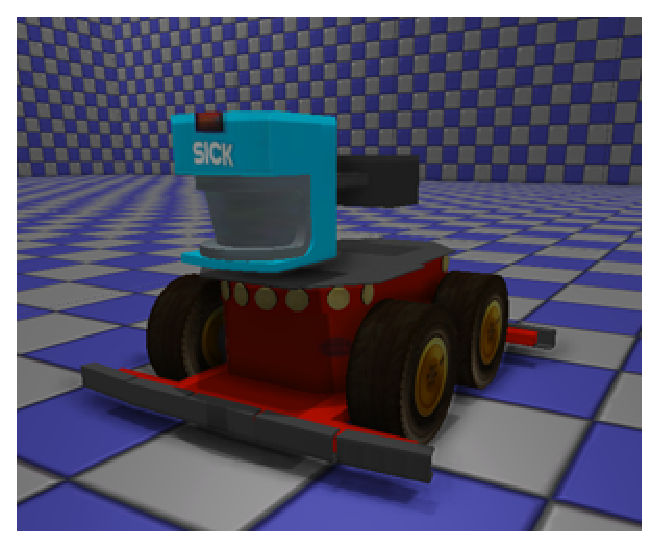
\includegraphics[width=4cm]{Figures/Robots/P3AT.eps}
\caption{Pioneer 3-AT (P3AT) in USARSim.}\label{fig:p3at}
\end{figure}




\subsubsection*{Low-level Navigation}
The ROS/USARSim interface allows the startup and the control of the default P3AT base controllers by directly sending velocity commands to the base. This task was performed using the following commands:
\begin{enumerate}
\item Bring up an environment in USARSim
\item \$ \texttt{roscore}
\item \$ \texttt{roslaunch usarsim usarsim.launch}
\item \$ \texttt{rosrun teleop\_twist\_keyboard teleop\_twist\_keyboard.py}
\end{enumerate}

In the first step, the user starts the environment in USARSim. If an environment is not up and running, passing messages between ROS and USARSim is not possible. The second step starts \texttt{roscore}, a collection of nodes and programs that are a pre-requisites of a ROS-based system. \texttt{roscore} must run in order for ROS nodes to communicate. The third step launches the \texttt{usarsim.launch} file. This launch file contains information necessary to connect ROS to the computer running the server (USARSim), to set up the appropriate robot (the P3AT in this case) at the correct location in the environment, to launch the proper ROS topics and to start the \texttt{RosSim} node. The last step starts the \texttt{teleop\_twist\_keyboard} node which sends velocity commands to the \texttt{RosSim} node through the computer keyboard. At this point, the P3AT can be controlled by keyboard teleop in the USARSim environment.

Figure~\ref{fig:teleop} illustrates the communication between the \texttt{RosSim} and the \texttt{teleop\_twist\_keyboard} nodes (in ovals). The keyboard inputs are converted in velocity commands and then communicated to the \texttt{RosSim} node on the topic \texttt{cmd\_vel}. \texttt{RosSim} publishes two topics for the odometry (\texttt{GndTruth} and \texttt{InsTest}), one topic to keep track of multiple coordinate frames over time \texttt{tf}, and a topic for the laser scanner (\texttt{lms200}).
\begin{figure}[h!]
\centering
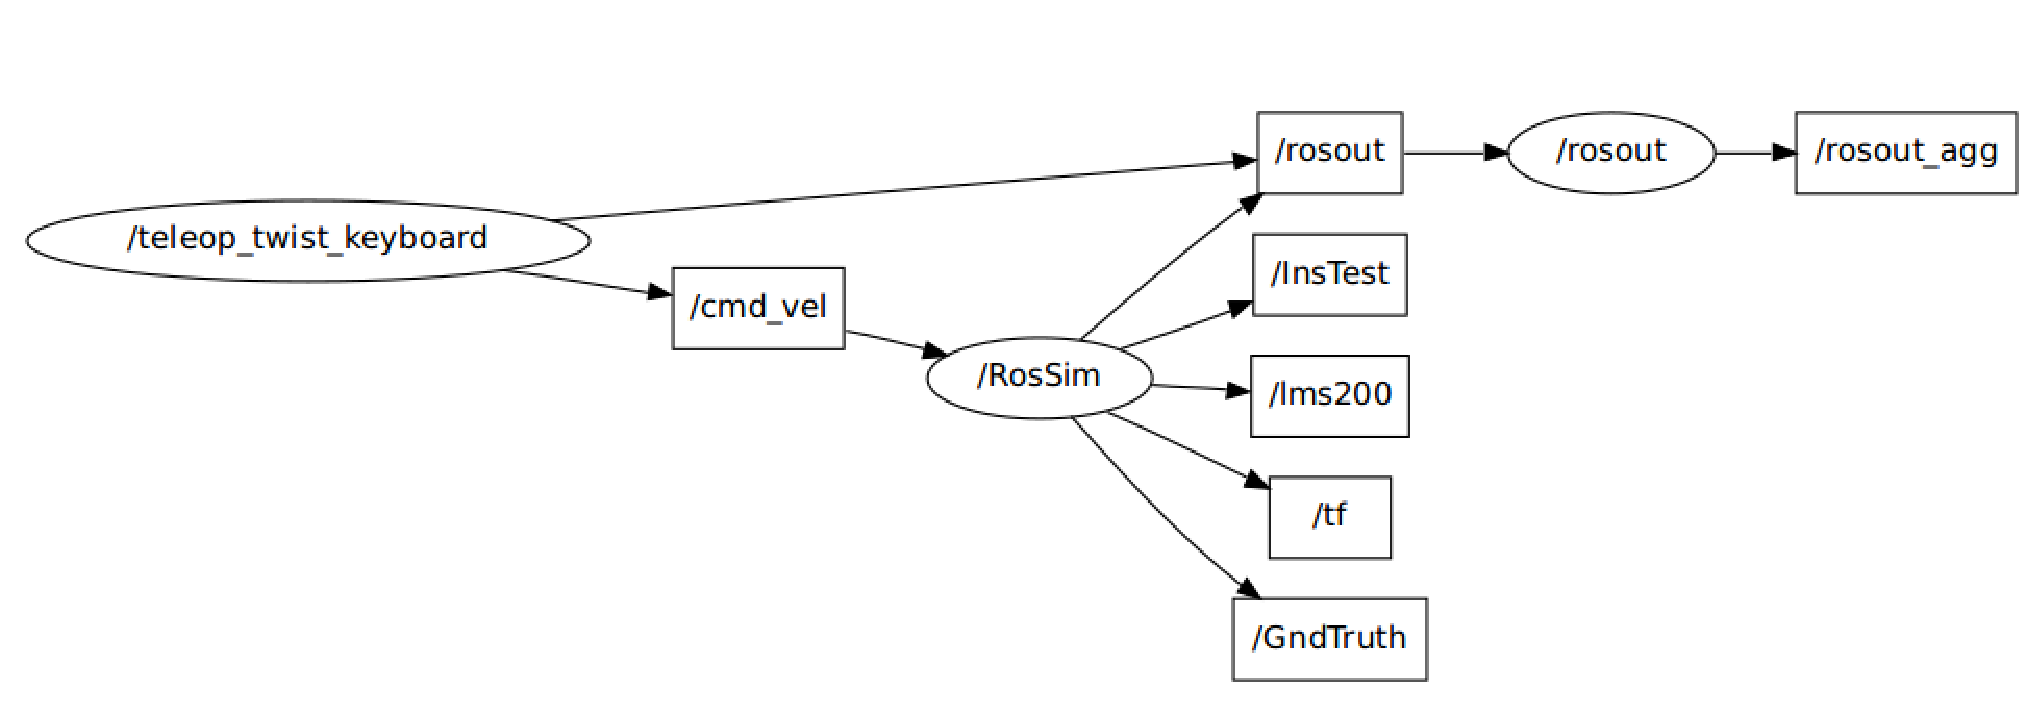
\includegraphics[width=9cm]{Figures/Misc/teleop-rossim-non-quiet.eps}
\caption{Mobile robot control at the lower level.}\label{fig:teleop}
\end{figure}

\subsubsection*{High-level Navigation}
This section describes how goals are sent using code to the P3AT to move to a particular location. Navigation at hight level is possible with the action specification for \texttt{move\_base}. This package provides an implementation of an action (\texttt{actionlib}) that, given a goal in the world, will attempt to reach it with a mobile base. The \texttt{move\_base} node links together a global and local planner to accomplish its global navigation task. 

\begin{figure}[h!]
\centering
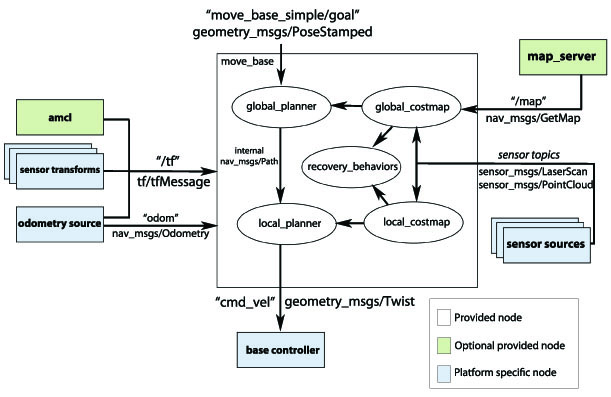
\includegraphics[width=9cm]{Figures/Misc/Navigation_Stack.eps}
\caption{Navigation stack setup.}\label{fig:navigation_stack}
\end{figure}
The \texttt{move\_base} node provides a ROS interface for configuring, running, and interacting with the navigation stack on a robot. The diagram in Figure~\ref{fig:navigation_stack} depicts a high-level view of the \texttt{move\_base} node and its interaction with other components of the navigation stack. The white components are required components that are already implemented, the green components are optional components that are already implemented, and the blue components must be created for each robot platform. 
%The blue components were created for the P3AT, enabling ROS to control the robot at lower and higher levels of the navigation stack.

Before running the \texttt{move\_base} node on the P3AT, localization, mapping and navigation information are filled in the \texttt{move\_base.launch} file:
\begin{itemize}
 \item [-] Localization uses map, laser data, and odometry to situate the robot in relation to the environment. The \texttt{amcl} and the \texttt{map\_server} nodes are necessary for robot localization. \texttt{amcl} is a probabilistic localization system for a robot moving in 2D and implements the KLD-sampling\cite{DIETER.IJRS.2003}. 
The \texttt{amcl} node is launched from the examples directory of the amcl package.
% and is included in \texttt{move\_base.launch} as one of its parameters.
\item [-] The \texttt{map\_server} node uses an a priori map generated by the \texttt{map\_saver} command-line utility. The generated map is stored in pair of files: the YAML file describes the map metadata and a reference to the image file that encodes the occupancy data. 
\item [-] The navigation stack uses costmaps to store information about obstacles in the world. A global costmap is used for creating long-term plans, and a local costmap is used for local planning and obstacle avoidance. Both costmaps need to follow some configuration options, stored in a third costmap file. Details on the costmaps are stored in YAML files.
\item [-] To compute velocity commands to send to the robot given a high-level plan, the navigation stack uses a base local planner. Information on the base local planner is stored in a YAML file which sets configuration options based on the specs of the robot. 
\end{itemize}

Once the \texttt{move\_base.launch} file is setup with the appropriate configuration options, the \texttt{move\_base} node can be started by using the following command:
\begin{itemize}
 \item [] \item \$ \texttt{roslaunch move\_base.launch}
\end{itemize}

-- Need rxgraph file to finish this section --

\subsection*{Robotic Arm Interface}
Steve
